\chapter{Literature Review and Related Work}
\label{chap:relatedworks}

In this chapter, describe other solutions/research that address the
same topic as your project. If you are working on a software project, create a
list of alternative solutions and analyze them in the competitor analysis section.
If you are working on a research project, describe your related work research in
the literature review section.

\section{Competitor Analysis}
\label{section:competitor-analysis}
\begin{enumerate}

    \item \textbf{Competitor Overview}
    \begin{enumerate}
        \item \textbf{Trello} \\
        Trello is a task management tool that uses boards, lists, and cards. It helps users organize tasks visually and move them through different stages. It is simple, flexible, and good for teams or individuals.  

        \begin{figure}[H]
            \centering
            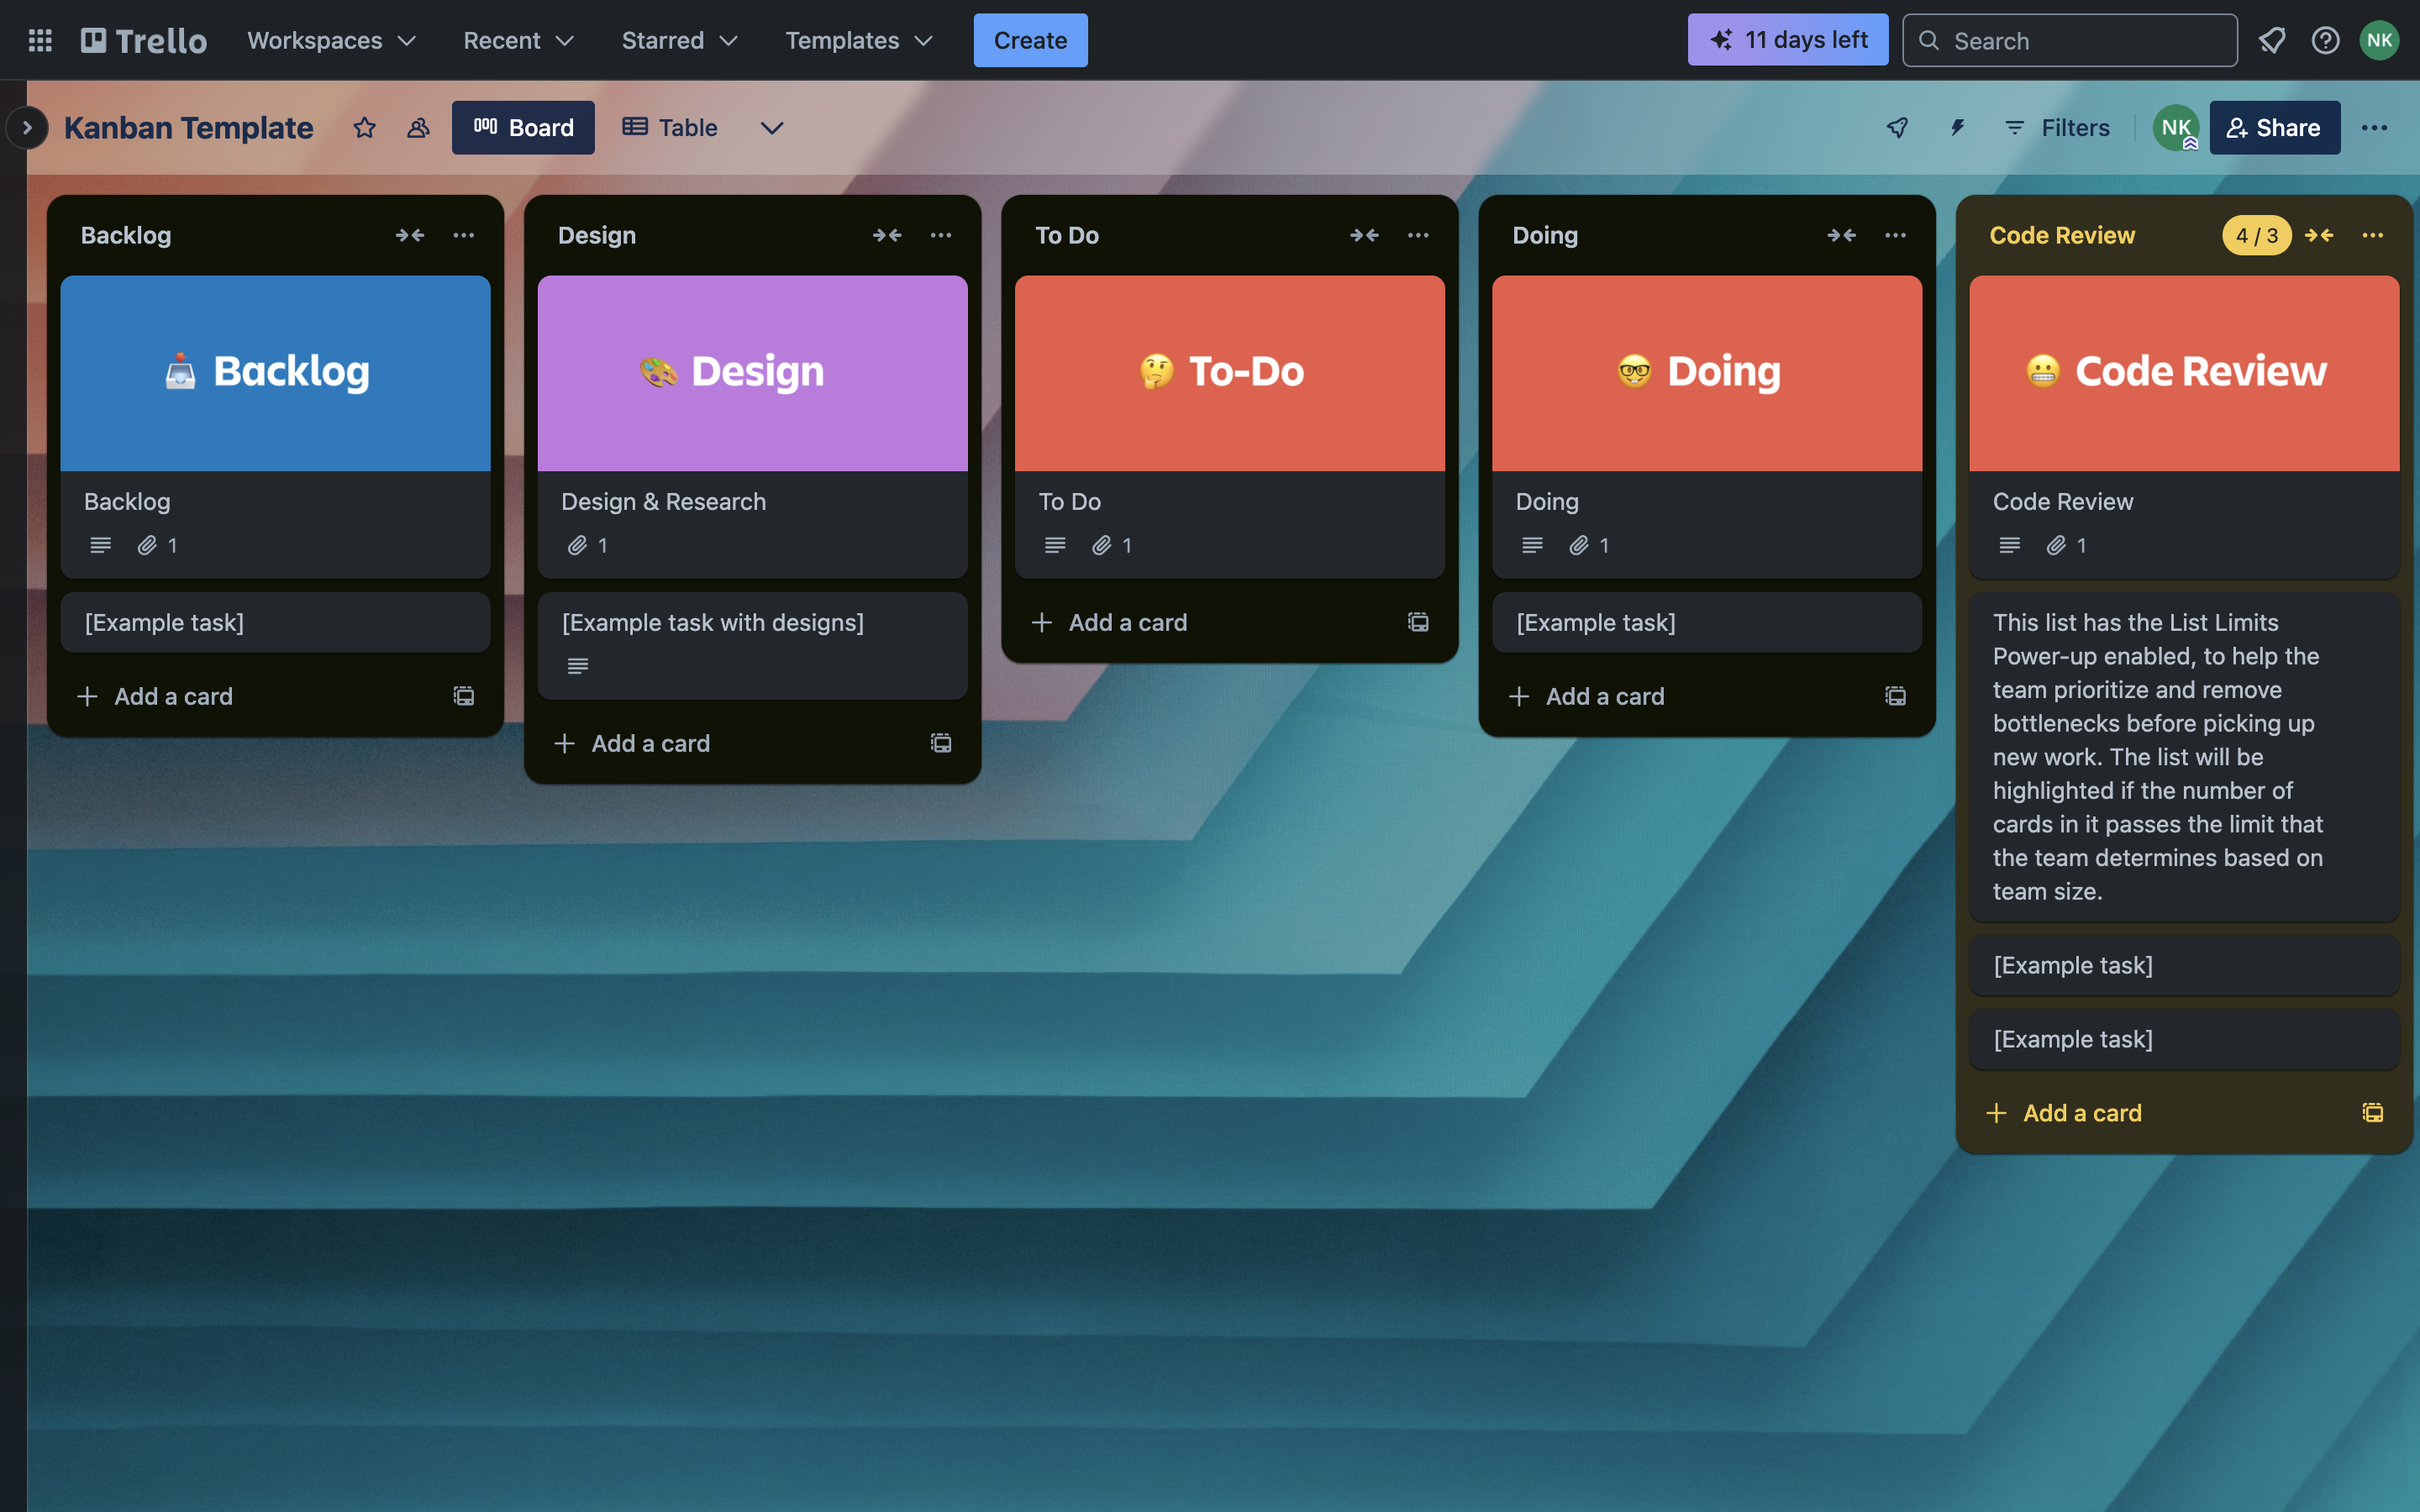
\includegraphics[width=0.6\textwidth]{examples/Trello.png}
            \caption{Trello}
        \end{figure}

        \item \textbf{Asana} \\
        Asana is a tool for managing projects and tasks. Users can create task lists, set deadlines, and track progress. It supports different views like lists, boards, and timelines, making it useful for teams working on complex projects.  

        \begin{figure}[H]
            \centering
            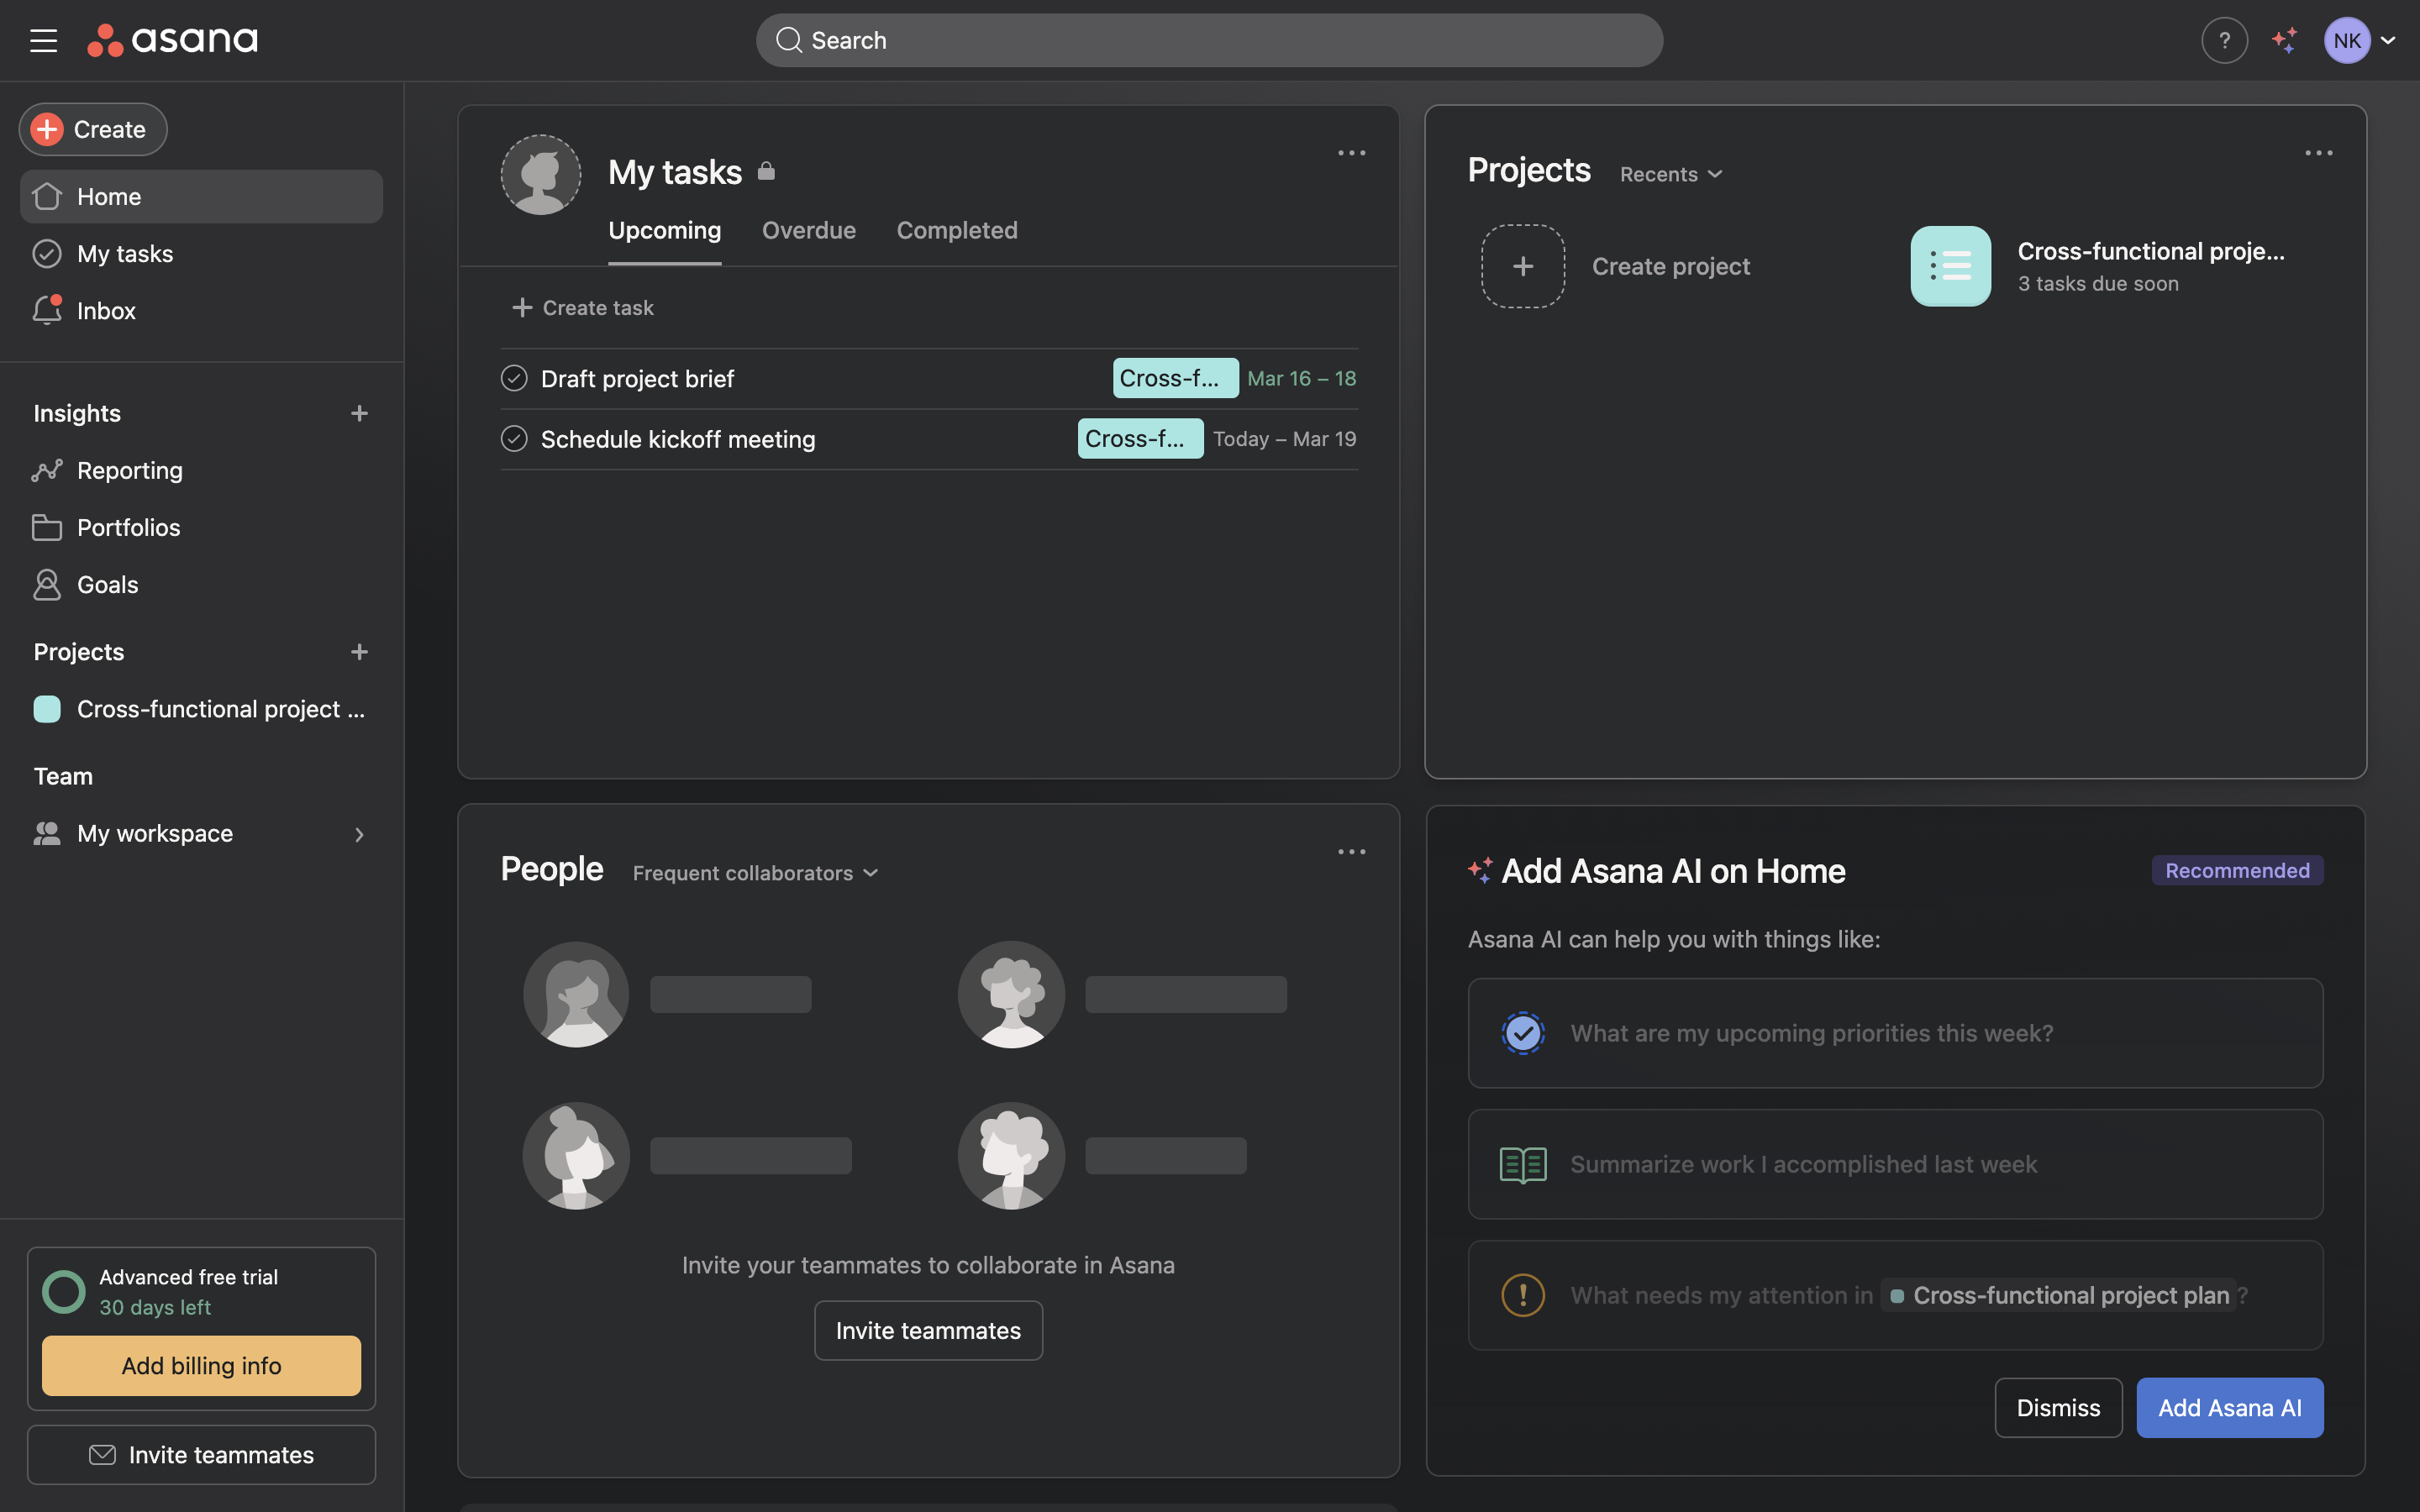
\includegraphics[width=0.6\textwidth]{examples/Asana.png}
            \caption{Asana}
        \end{figure}

        \item \textbf{Monday.com} \\
        Monday.com is a work management tool that helps teams plan and track work. It has customizable workflows, automation, and visual dashboards. Teams can organize tasks in a way that fits their needs.  

        \begin{figure}[H]
            \centering
            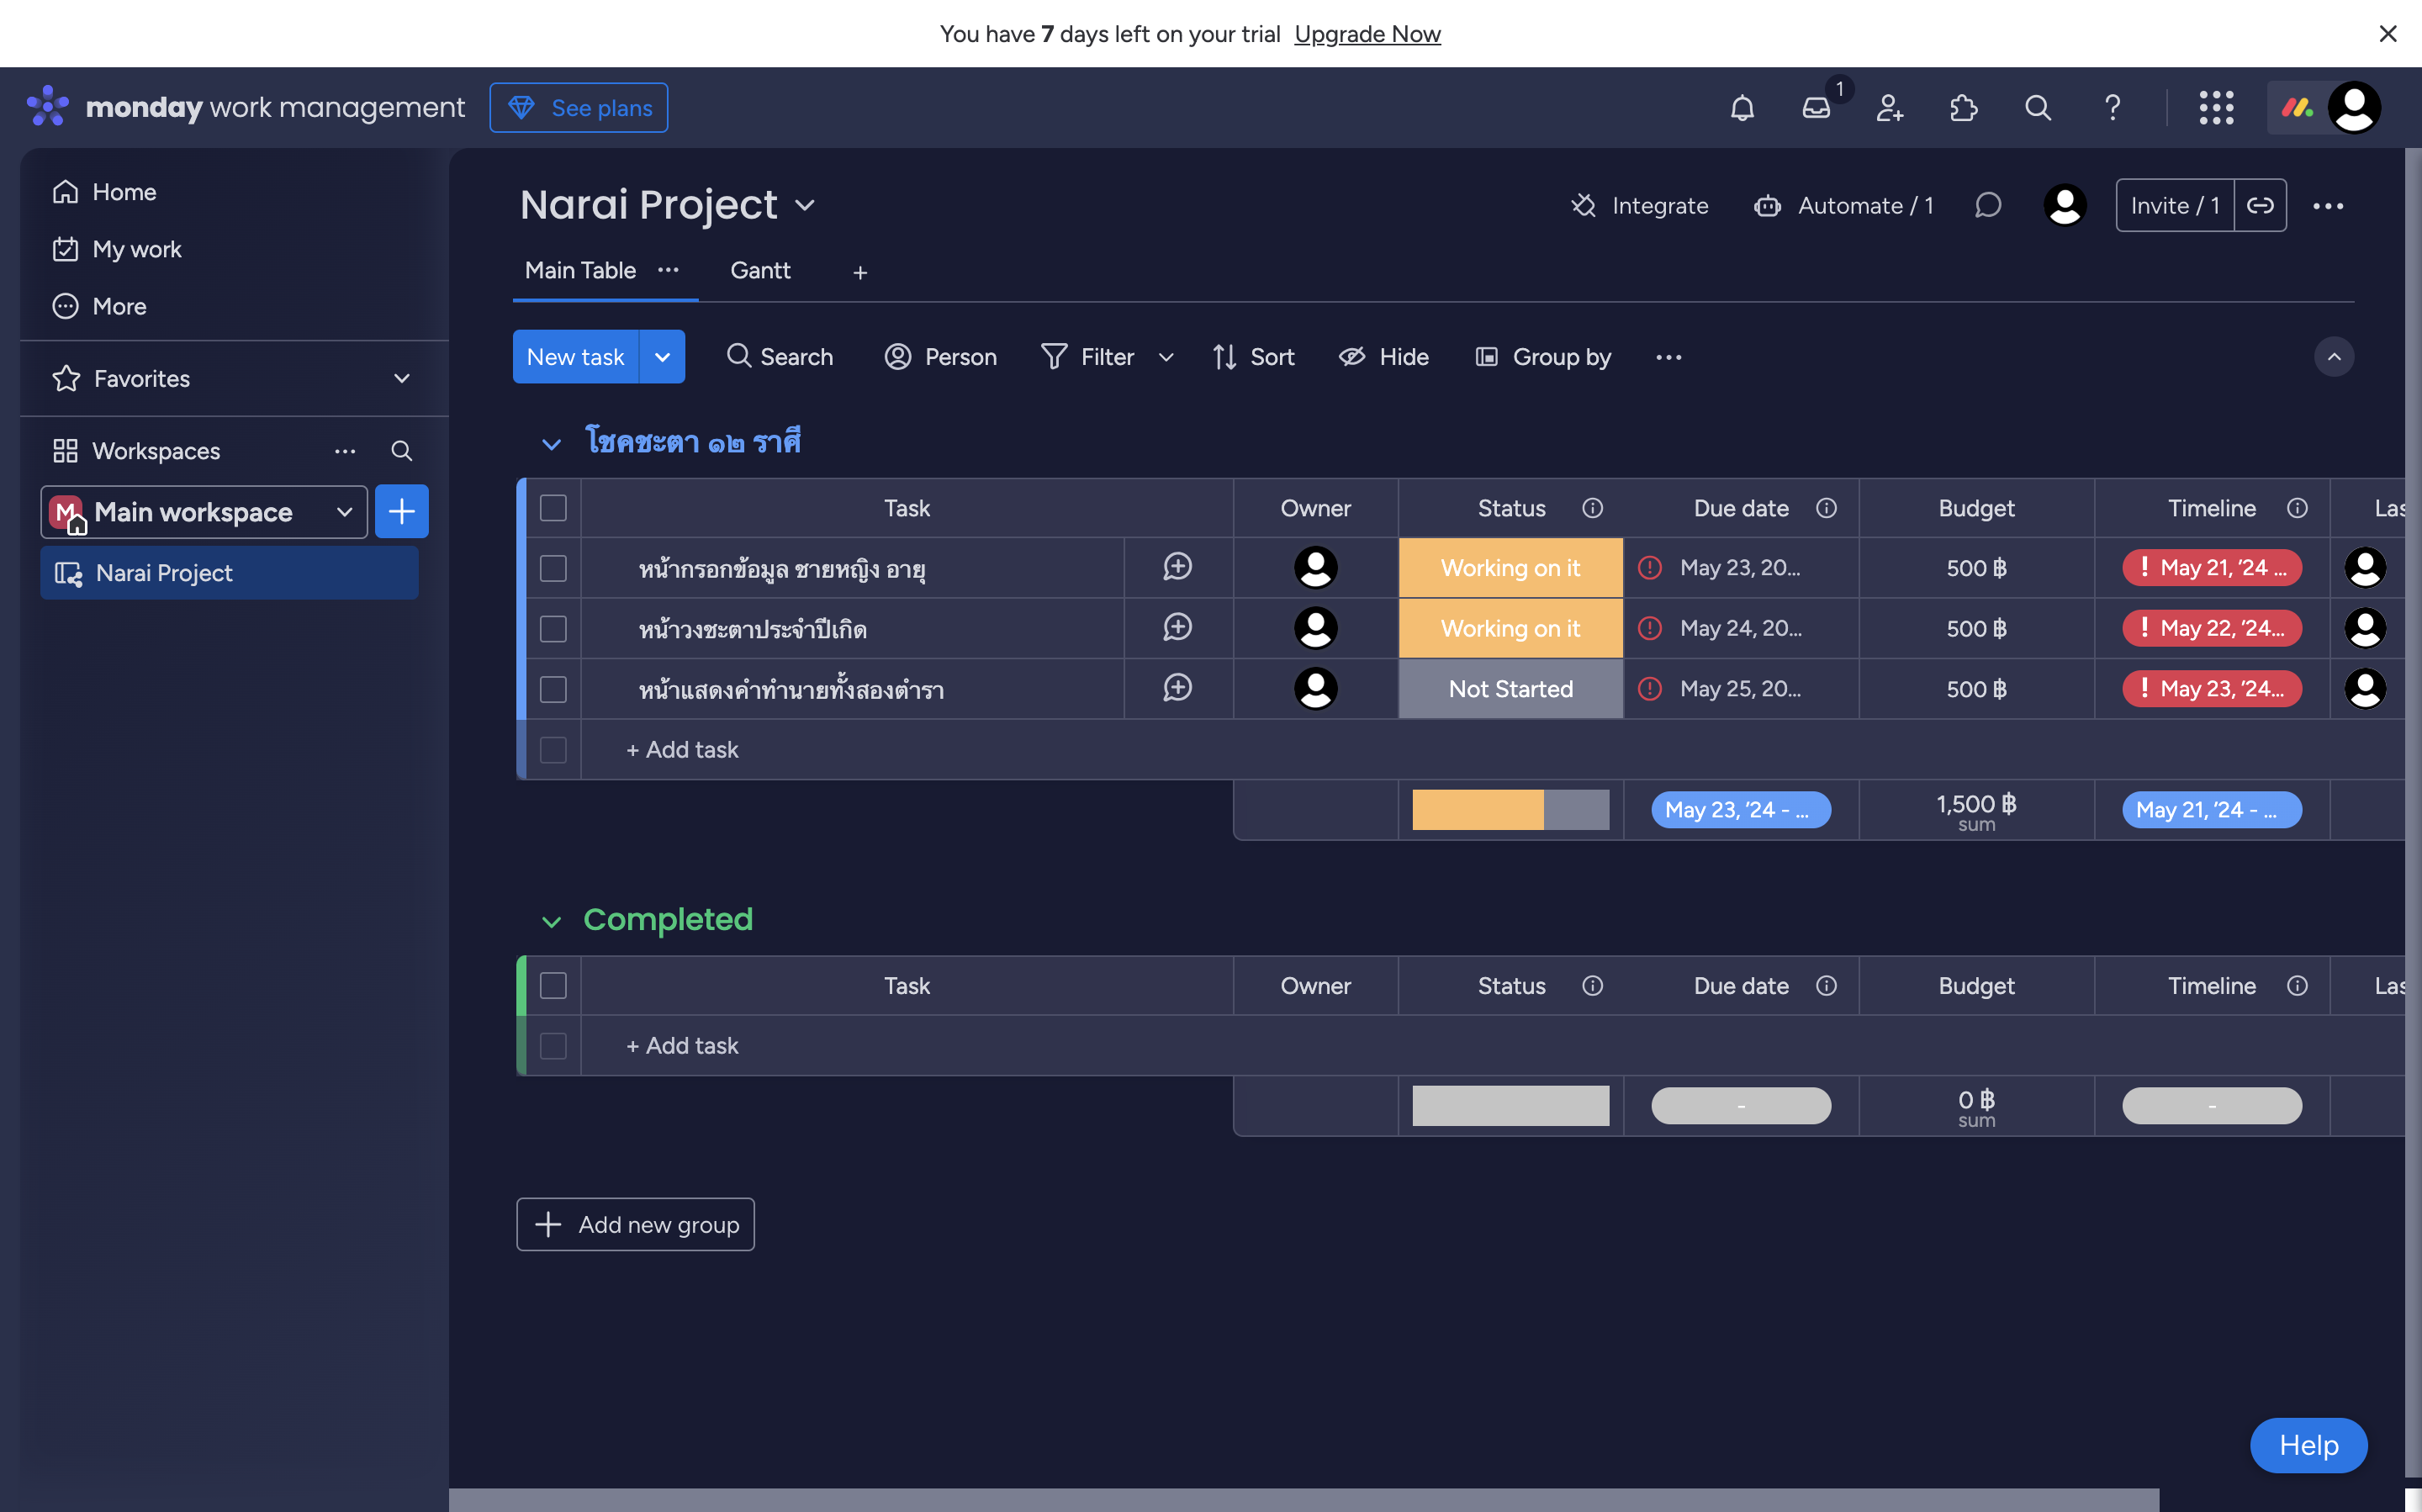
\includegraphics[width=0.6\textwidth]{examples/Monday.png}
            \caption{Monday.com}
    \end{figure}

    \item \textbf{Habitica} \\
    Habitica is a habit tracker that turns daily tasks into a game. Users complete tasks to earn rewards and level up. It makes productivity fun by using game elements to build good habits.  

    \begin{figure}[H]
        \centering
        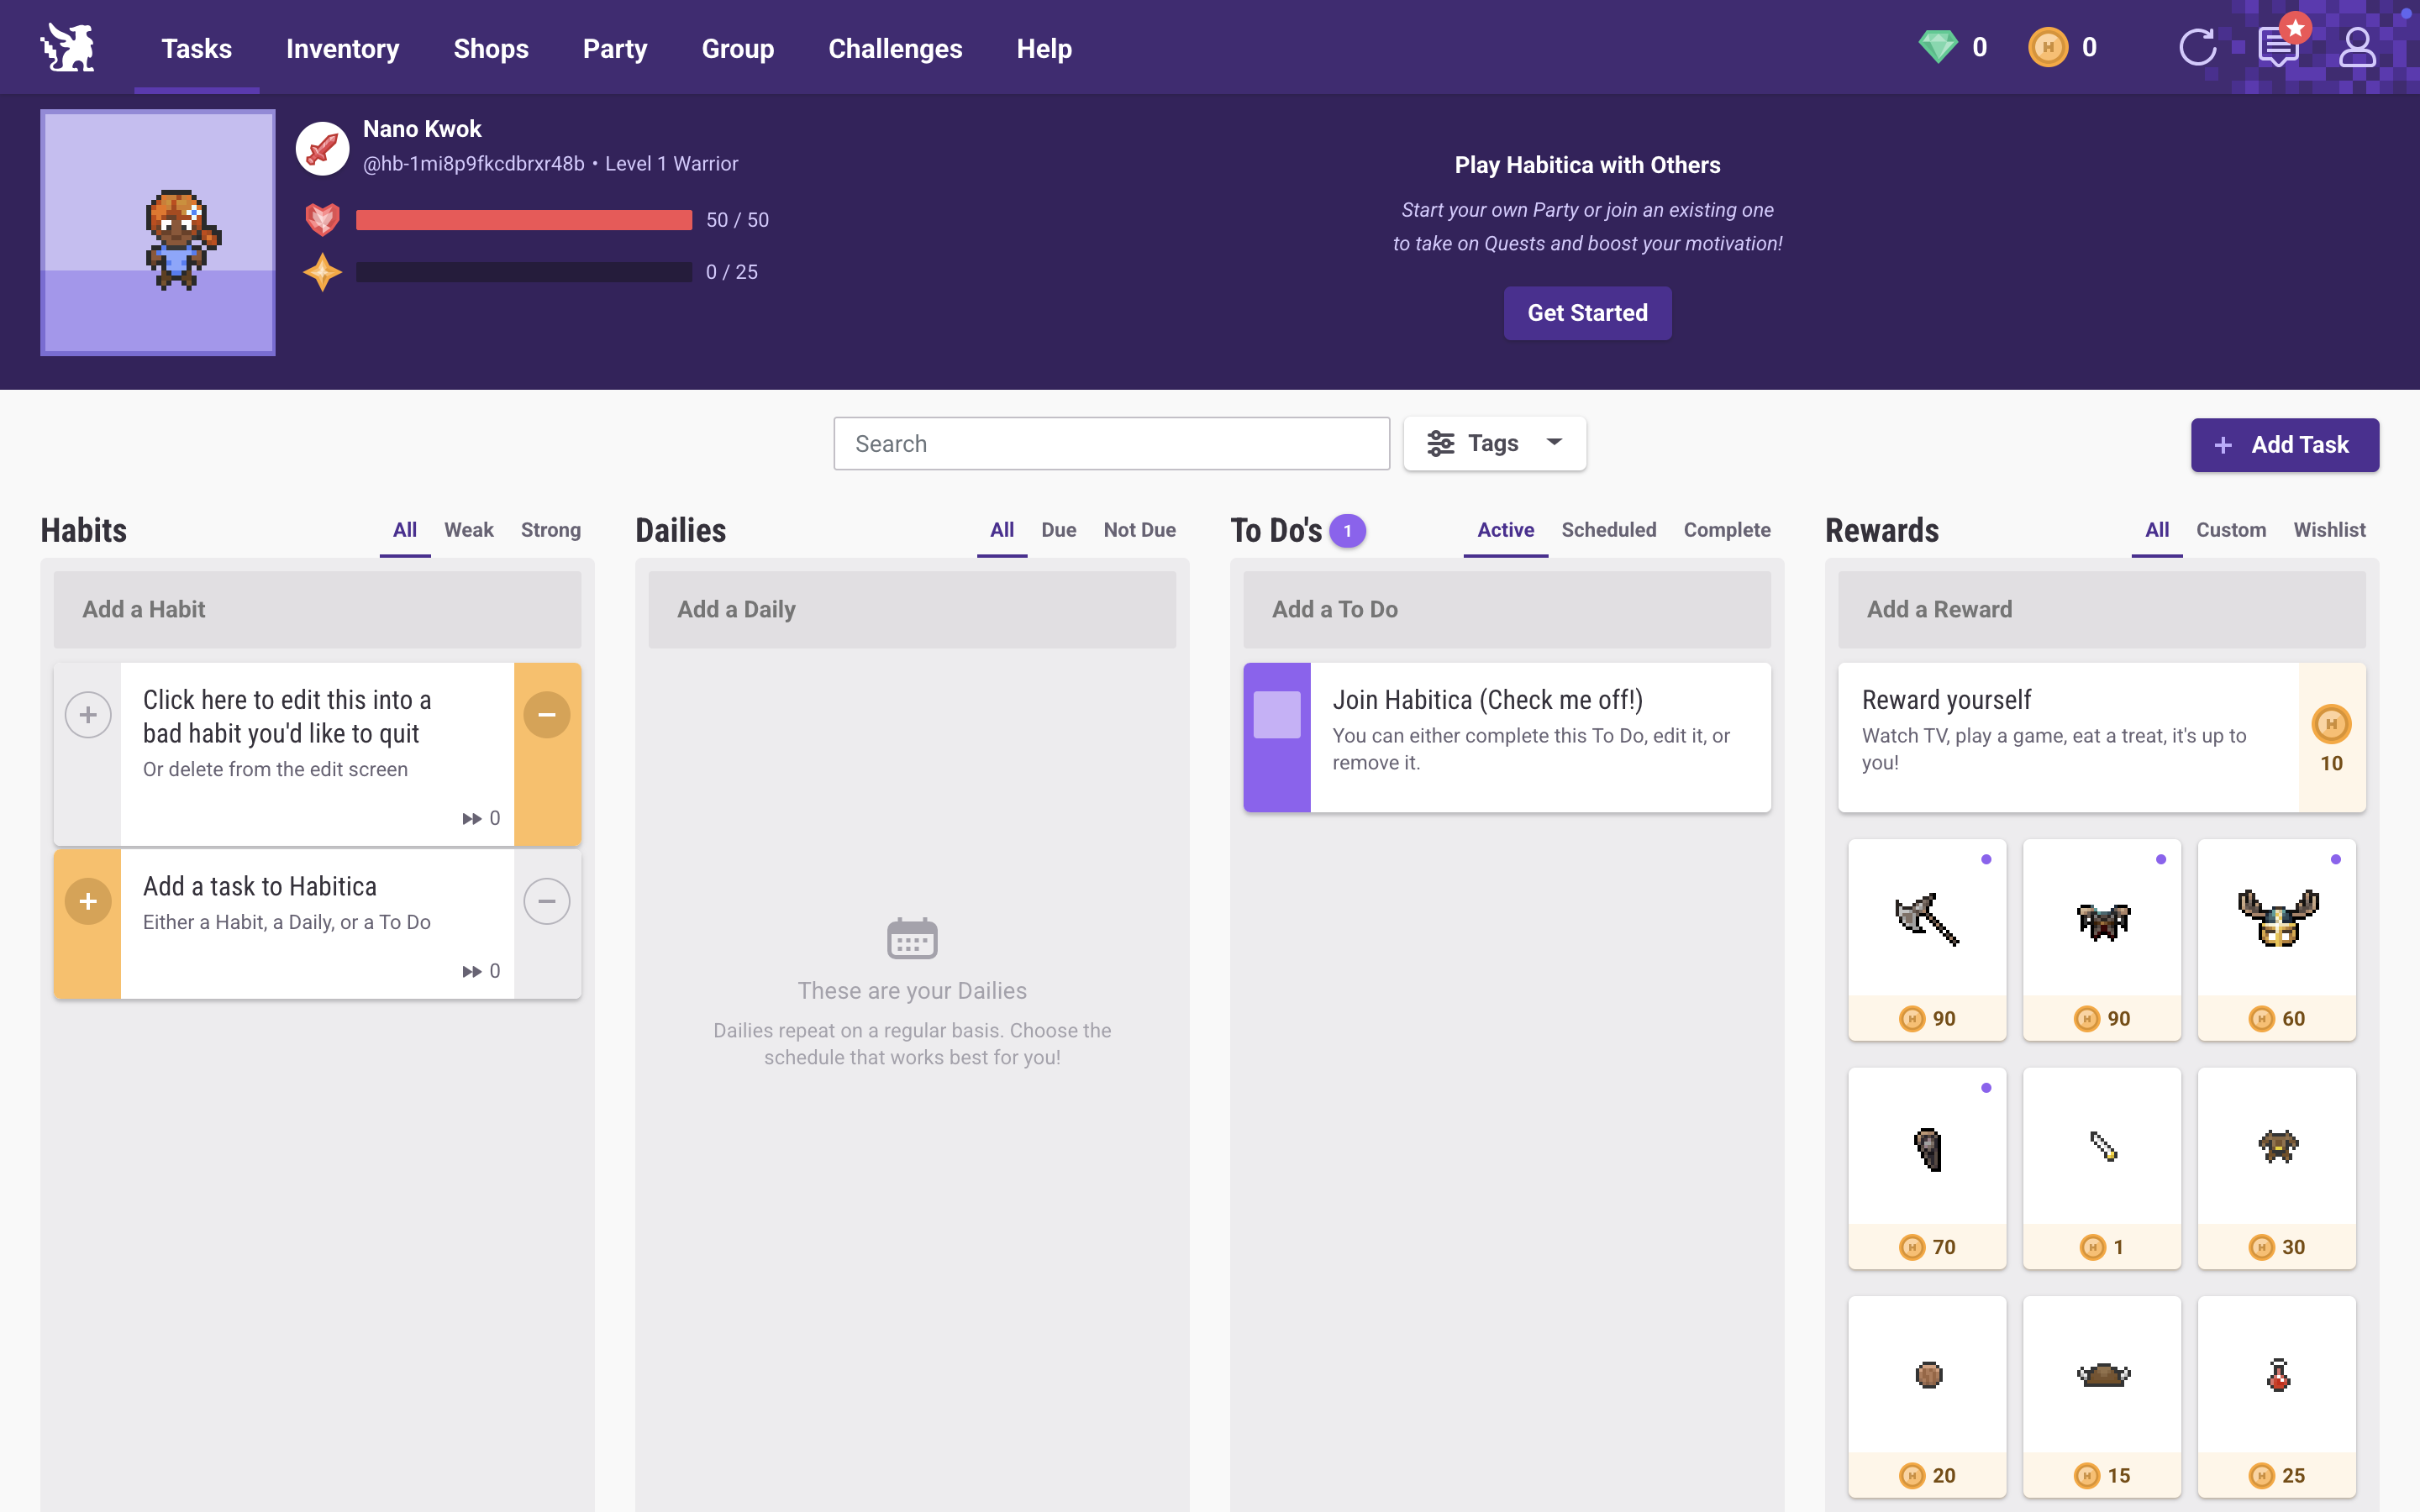
\includegraphics[width=0.6\textwidth]{examples/Habitica.png}
        \caption{Habitica}
    \end{figure}

    \item \textbf{Fucumon} \\
    Fukumon is a gamified productivity app that gives rewards for completing tasks. It helps users stay motivated by making work feel more enjoyable and engaging.  

    \begin{figure}[H]
        \centering
        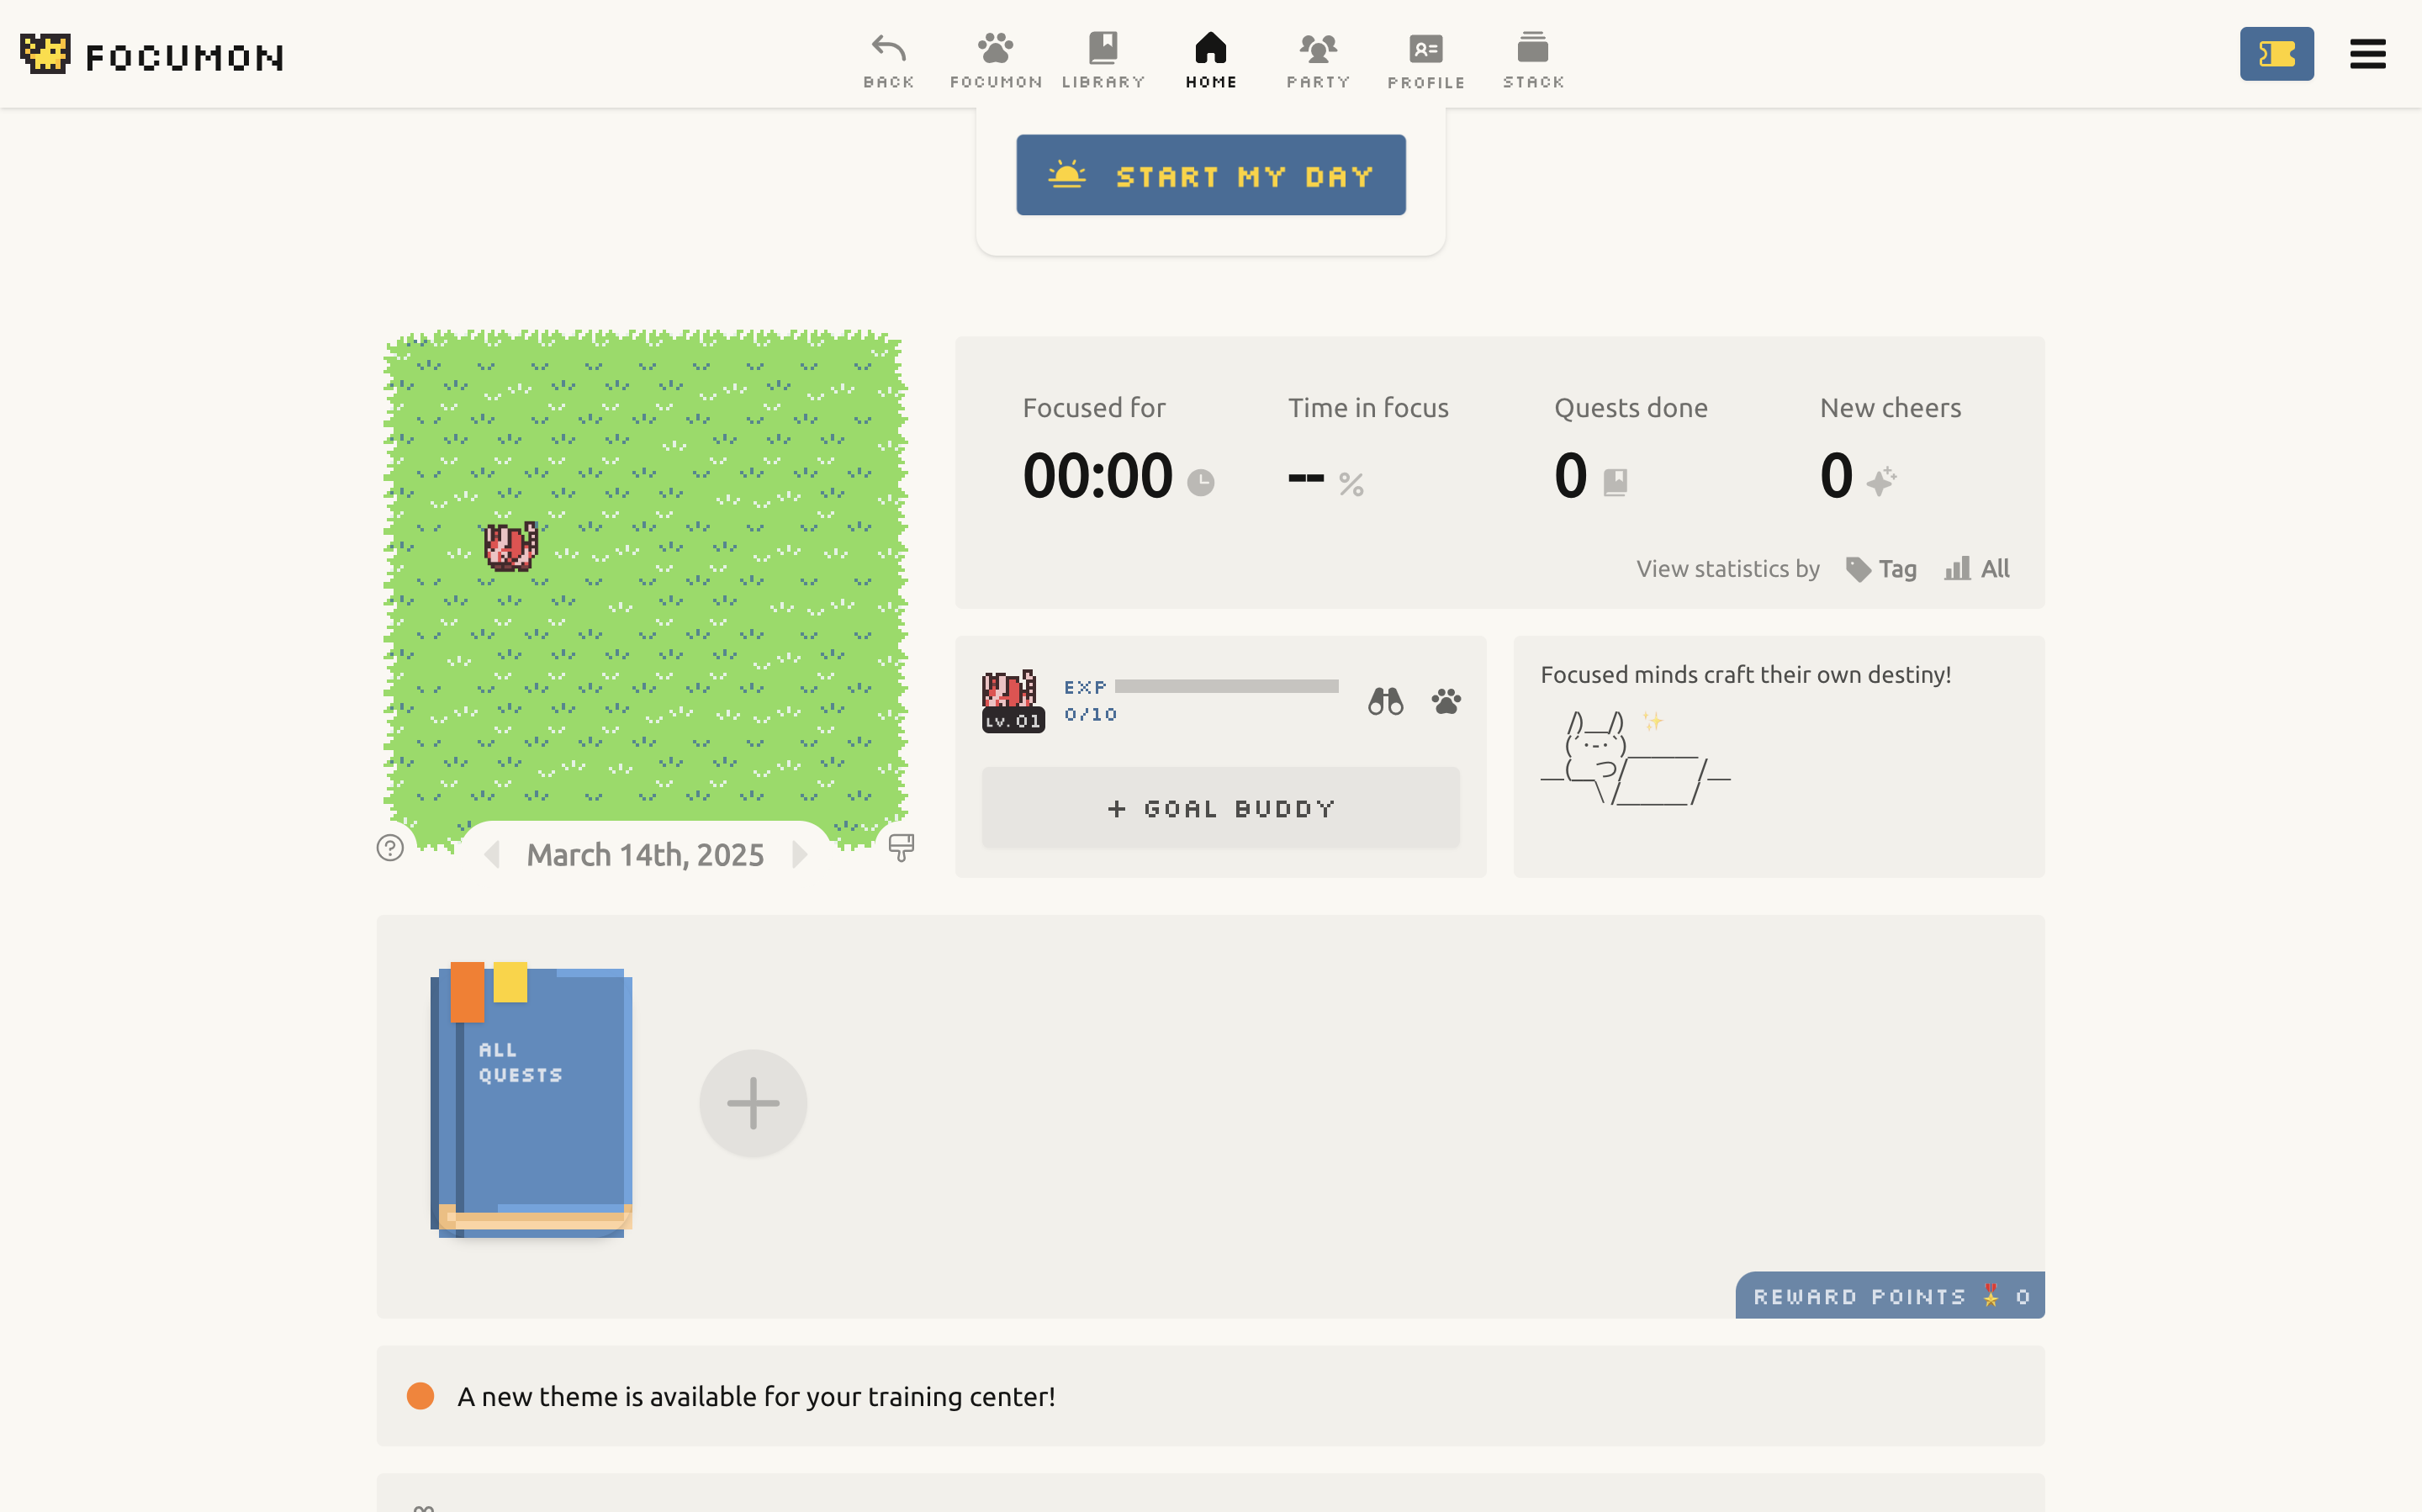
\includegraphics[width=0.6\textwidth]{examples/Fucumon.png}
        \caption{Fukumon}
    \end{figure}   
    \end{enumerate}
    \item \textbf{Product Feature Comparison}

    \noindent\begin{center}
    \begin{table}[ht]
        \centering
        \footnotesize 
        \rowcolors{2}{white}{gray!10}
        \begin{tabularx}{\textwidth}{|>{\raggedright\arraybackslash}X|>{\raggedright\arraybackslash}X|>{\raggedright\arraybackslash}X|>{\raggedright\arraybackslash}X|>{\raggedright\arraybackslash}X|>{\raggedright\arraybackslash}X|>{\raggedright\arraybackslash}X|}        
            \hline
            \rowcolor{gray!70}
            Features & WorkQuest & Trello & Asana & Monday.com & Habitica & Fukumon \\
            \hline
            Task Management & Kanban boards, automation & Kanban boards & Task lists & Custom workflows & Daily tasks & To-do lists \\
            \hline
            Gamification & XP, rewards & No & No & No & RPG-style game & Rewards system \\
            \hline
            AI Feedback & Yes & No & No & No & No & No \\
            \hline
            Collaboration Task assignments & Chat, shared tasks & Boards, comments & Task assignments & Team dashboards & No & Shared tasks \\
            \hline
            Reward System & Leader board, badges & No & No & No & Coins, items & Points, achievements \\
            \hline
            Customization & Workflows, themes & Boards, labels & Templates & Dashboards & No & Task settings \\
            \hline
        \end{tabularx}
        \caption{Feature Comparison Among Competitors}
        \label{tab:feature-comparison}
    \end{table}
    \end{center}

\item \textbf{Product Marketing Comparison}
    \begin{enumerate}
        \item \textbf{Social Media \& Advertising}
        \begin{itemize}
            \item Trello, Asana, and Monday.com focus on business users.
            \item Habitica and Fukumon highlight gamified motivation.
            \item WorkQuest focus on team engagement.
        \end{itemize}
        
        \item \textbf{Website \& Brand Voice}
        \begin{itemize}
            \item Trello and Asana promote workflow efficiency.
            \item Habitica and Fukumon market personal growth.
            \item WorkQuest focuses on gamified collaboration.
        \end{itemize}
    \end{enumerate}

    \item \textbf{SWOT Analysis}
    \begin{enumerate}
        \item \textbf{Strengths}
        \begin{itemize}
            \item Unique gamified approach with AI feedback.
            \item Focuses on team collaboration.
            \item Engaging reward-based mechanics.
        \end{itemize}
        
        \item \textbf{Weaknesses}
        \begin{itemize}
            \item New to the market.
            \item Requires user adaptation to gamification.
        \end{itemize}

        \item \textbf{Opportunities}
        \begin{itemize}
            \item Increasing demand for gamified productivity.
            \item Schools and companies may find it useful.
        \end{itemize}

        \item \textbf{Threats}
        \begin{itemize}
            \item Strong competition from established platforms.
            \item Users may hesitate to switch tools.
        \end{itemize}
    \end{enumerate}

    \item \textbf{Market Positioning}
    \begin{enumerate}
        \item WorkQuest stands at the intersection of gamification and team collaboration.
        \item Differentiates from competitors by integrating AI feedback and engagement.
    \end{enumerate}

\end{enumerate}

% \begin{figure}[h]
%     \centering
%     \includegraphics[width=0.5\textwidth]{examples/asana-competitive-landscape.jpg}
%     \caption{Competitive Landscape by Asana}
% \end{figure}

% Refer to an article "How to create a competitive analysis (with
% examples)" by Asana. You can use the Competitor Landscape (left image) or
% Competitor Analysis Framework (right image) for your project.

\section{Literature Review}
\label{section:literature-review}
    Task management plays an important role in work productivity, but many teams face challenges with staying engaged, avoiding procrastination, and improving collaboration. Traditional task management systems can sometimes feel rigid, which can lead to difficulties in maintaining motivation over time.

    In response to these challenges, gamification has emerged as a promising strategy to enhance engagement and performance by integrating game-like elements—such as goals, rewards, competition, and collaboration—into workplace settings. Research consistently shows that gamification provides team members with a sense of autonomy, competence, and relatedness, thereby creating a fun and engaging work environment \cite{ncbi:pmc10905147}. Moreover, practical advantages have been demonstrated across various performance metrics, supported by evidence from real-life case studies. \cite{Employee:Gamification}

    WorkQuest introduces a unique approach to task management by integrating gamification elements—specifically "boss fight" mechanics—and AI performance evaluation. In this system, Users collaborate to complete tasks that weaken and ultimately defeat a boss, adding a layer of strategic engagement. AI-driven analysis provides personalized performance feedback, ensuring that users receive tailored insights to improve efficiency.

    The application of gamification involves the use of goal-setting for direction, challenges to maintain interest, rewards to reinforce success, and feedback to guide improvement. These elements work synergistically to keep participants engaged, boost performance, and align intrinsic and extrinsic motivations. \cite{Game:Reward}

    Numerous studies have demonstrated the benefits of gamification in a variety of contexts. For example, research by Juho Hamari (2014) reviewed the impact of gamification across sectors and found that it consistently improves user engagement, productivity, and satisfaction by employing feedback loops, competition, and goal-setting as effective motivators. \cite{6758978}

    In the context of task management, gamification has been shown to improve productivity, collaboration, and task completion rates by transforming routine tasks into more engaging and motivating activities.

    Moreover, gamification has been shown to promote teamwork and collaboration. Deterding et al. (2011) emphasize that gamified systems enhance group dynamics by incorporating features like team challenges, leaderboards, and shared rewards, which encourage users to collaborate, share knowledge, and work together toward common goals. This approach improves collective productivity and communication within organizations. \cite{gamification:designElement}

    We are gamifying a task management application using a boss fight mechanic to increase engagement. Boss fights in video games are pivotal moments designed to challenge players and heighten engagement. These encounters often require players to utilize all the skills and strategies they've acquired, serving as ultimate tests of their abilities. Successfully overcoming a boss fight provides a strong sense of accomplishment, reinforcing player motivation and progression \cite{toxigon:bossFight}.

    In addition to enhancing motivation, boss fights create memorable emotional experiences by evoking feelings ranging from excitement and anticipation to frustration and relief. The atmosphere during boss encounters—shaped by music, sound effects, and visual design—further enhances immersion, making these battles feel more epic and impactful. \cite{toxigon:bossFight}

    Beyond entertainment, the concept of boss fights has also been explored in gamified learning environments. Research suggests that boss fights in educational settings can serve as powerful motivational tools, encouraging students to apply their knowledge and problem-solving skills in high-stakes scenarios. By integrating boss fights into gamified learning, educators can create more engaging and rewarding experiences, similar to how video games challenge and reward players \cite{gamification:Education}.

    Not only traditional boss fights, but we also offer a boss collection feature that can further enhance engagement. Rewarding players for defeating bosses and introducing a rotational or exclusive collection system leverages FOMO (Fear of Missing Out) to drive participation. This approach has been successfully used in games like Fortnite and Animal Crossing to sustain player interest and encourage long-term engagement \cite{medium:FOMO}. While some research highlights the potential risks of FOMO in gaming, including compulsive behaviors, when implemented responsibly, it serves as a powerful tool to keep players engaged and invested in the experience \cite{FOMO:1} \cite{FOMO:2}.

    While gamification serves as an essential engagement strategy, the integration of AI provides a complementary approach to enhance user experience through personalized feedback and performance evaluation. In WorkQuest, we integrate AI not only for gamification but also to provide personalized feedback to users. This helps individuals understand how they can improve and enables teams to assess overall performance. Unlike traditional evaluation methods, AI-driven systems analyze large datasets to measure individual contributions, track task efficiency, and offer tailored recommendations for improvement.

    To effectively achieve these goals, we utilize multiple criteria for performance evaluation, including Work Speed Analysis, Strength Identification, Work Quality Evaluation, Teamwork Evaluation, Diligence Scoring, and Workload Tracking. Furthermore, we employ K-Means clustering to determine user roles, which is integrated with Q-learning to generate personalized feedback and task recommendations. By organizing users based on their performance patterns, this approach ensures that the feedback provided is accurate, targeted, and conducive to individual growth and team efficiency.

    Building upon these evaluation criteria, recent advancements in AI, particularly in Natural Language Processing (NLP) and Machine Learning (ML), have enhanced transparency, fairness, and personalized feedback mechanisms. For instance, NLP models like BERT are capable of contextual understanding, improving the quality of feedback provided to users. \cite{AI:humanResource}

    Moreover, techniques such as K-Means clustering and Reinforcement Learning (Q-learning) have proven effective in generating personalized task recommendations and role identification. For example, Q-learning-based differential evolution with K-Means clustering enhances clustering mechanisms for user segmentation, allowing for targeted feedback and improved collaboration. This approach is particularly useful in dynamic environments where user performance varies over time. \cite{PlusOne:Q-learingWithK-means}

    However, in WorkQuest, performance evaluation is conducted only at the end of a project, ensuring a comprehensive assessment of contributions and outcomes. While AI enables real-time data analysis, the structured end-of-project assessment ensures that feedback is holistic and reflective of overall performance.

    As organizations increasingly adopt AI-driven performance evaluation, balancing automation with human oversight will be essential to ensure fairness, adaptability, and long-term success in collaborative work environments.

    Overall, the integration of gamification and AI-driven feedback mechanisms represents a promising evolution in task management. By combining these strategies effectively, it is possible to create engaging, efficient, and adaptable systems that enhance productivity and satisfaction across various contexts.



